\chapter{A Dynamic Programming Approach}

We import LiDAR data and shape-file that contain geometric information of the location for each sidewalk. Instead of analysis the texture difference between desire sidewalk and non-sidewalk feature, we treat it as the ribbon-like feature and try to segment them base on their growth from start point. 

% \begin{figure}[H]
%     \centering
%     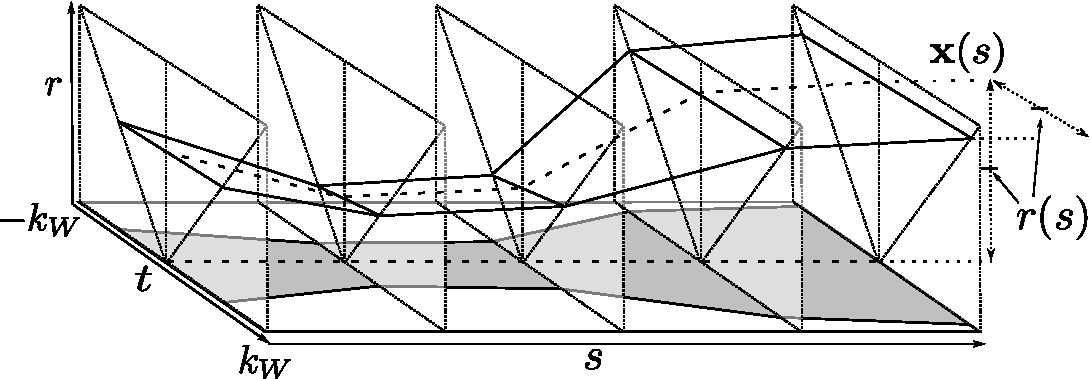
\includegraphics[width=\textwidth]{Figures/ribbon-3d.pdf}
%     \caption[3D Ribbon Image]{An illustration of the parameters for a ribbon; the $r$ axis captures the thickness of the ribbon and the $s$ axis captures the distance along the initial ribbon. The $t$ axis records horizontal displacements from the initial ribbon's medial curve.}
%     \label{fig:ribbon_3d}
% \end{figure}

\begin{figure}[htb]
    \centering
    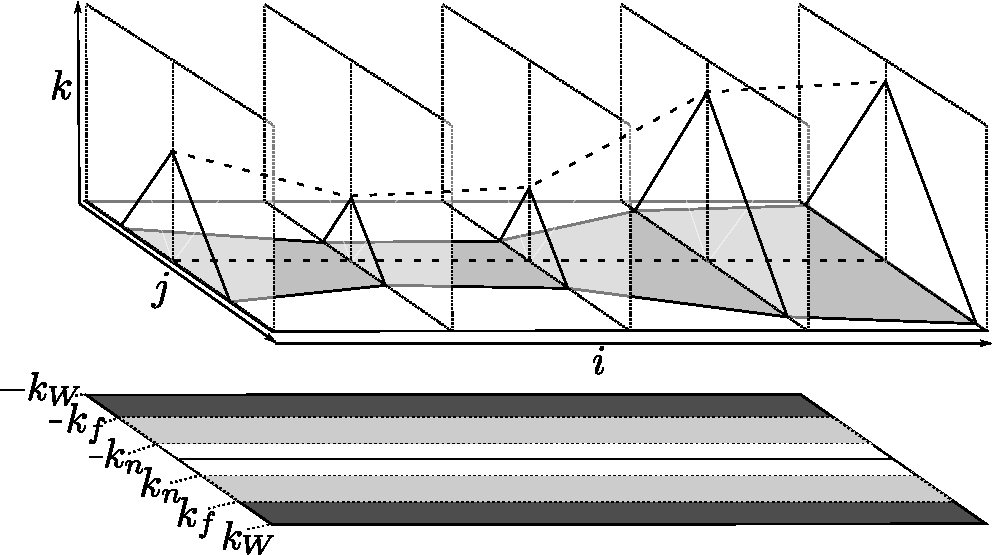
\includegraphics[width=0.95\columnwidth]{Figures/ribbon-3d-combined.pdf}
    \caption[3D Ribbon Image]{An illustration of the parameters for a ribbon: (top) the $k$ axis captures the thickness of the ribbon and the $i$ axis captures the distance along the initial ribbon, the $j$ axis records horizontal displacements from the initial ribbon's medial curve; (bottom) the boundaries of the ribbon must lie within $\pm \MaxDistance{}$, pixels within $\pm \MinRadius{}$ of the center are probably part of the ribbon and pixels further than $\pm \MaxRadius{}$ are likely negative. }
    \label{fig:ribbon_3d}
\end{figure}

\section{The Ribbon Image}

In order to simplify the problem, we first create a straightened "ribbon" image in which the sidewalk runs in a straight line, even if the original sidewalk if curved.
We represent a ribbon of length $L$ using parameters along and orthogonal to a medial curve $\mathbf{x}(s)$, where $s \in [0, L]$. The ribbon image is the set of all points within a perpendicular distance $r(s)$ to the medial curve.

A second parameter, which we call $t$, is measured in a direction orthogonal to the curve.  
We define ribbon coordinates $\mathbf{x}(s, t) = \mathbf{x}(s) + t\mathbf{n}(s)$, where $\mathbf{n}(s)$ is a vector perpendicular to the medial curve at position $s$, which can be obtained by rotating the curve's tangent vector $\dot{\mathbf{x}}(s)$ by 90 degrees. 


In practice we represent the curve $\mathbf{x}(s)$ discretely as an arc-length re-sampled set of points $\mathbf{x}_s,$ for $s=0,1,...,L-1$ from poly-line features that are read from a GIS file. The points are sampled at an arc-length distance of about one pixel between each point, and then Laplacian smoothing is applied in order diffuse the curvatures along the re-sampled poly-line.  
We use a secant to estimate the tangent to the curve,
\[\dot{\mathbf{x}}_s = \left[\begin{array}{c} \dot{x}_s \\ \dot{y}_s \end{array}\right]= \frac{\mathbf{x}_{s+1}-\mathbf{x}_{s-1}}{||\mathbf{x}_{s+1}-\mathbf{x}_{s-1}||} \] and rotate it ninety degrees counter-clockwise in order to find a direction  $\mathbf{n}_s$, so that 
\[\mathbf{n}_s = \left[\begin{array}{c} -\dot{y}_s \\ \dot{x}_s \end{array}\right]. \]

\begin{figure}
    \centering
    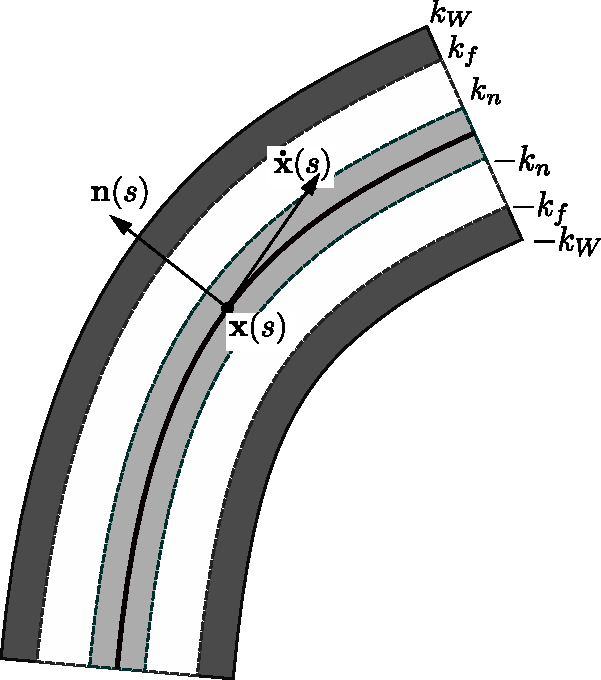
\includegraphics[width=\textwidth]{Figures/sw-figure.pdf}
    \caption[2D Ribbon Image]{A demonstration of the parameters for a ribbon in 2D. Where $k_n$ indicates a parameter that describes the radius of the medial curve that we considered to be part of the ribbon, $k_f$ is a distance from the medial curve that we considered very unlikely to be part of the ribbon, and $k_W$ is the maximum width of the ribbon image.}
    \label{fig:2d_ribbon}
\end{figure}

As shown in \ref{fig:2d_ribbon}, we assume that there is some uncertainty in the position $\mathbf{x}_s$ of the medial curve and also uncertainty in the radius $r_s$ of the discredited ribbon, but that there is range of distances $t \in 0\dots k_n$ from the medial curve which we can accept labeling as positive examples that are within the ribbon, and that there is some range of distances $t \in k_f\dots k_W$ which we can accept labeling as negative sample, and finally a range $t\in (k_n+1)...(k_f-1)$ of distances that are possible locations of the ribbon's boundary.  Therefore, when searching for improved medial curves and radii of the ribbon, we can consider a discrete range of offsets $t=-k_W,..., k_W$ chosen to be wide enough that true ribbon image itself likely fits entirely within the grid of input negative samples along its edges.  

The orthorectified color image $\image(x,y)$
records the color at the point $x,y$ in the image plane.
Then $\image(\mathbf{x}_{s,t}),$ is a warped version of the image in which the ribbon is centered on a single strip at $t=0$.
The situation is illustrated in \ref{fig:ribbon_3d}.  
In this warped image, we can estimate the amount $t_s$ to shift the ribbon's center in the $t-$axis, which is orthogonal to the curve,  and also the amount the radius $r_s$ so that the  ribbon at each row is in columns $(t_s - r_s)\dots(t_s+r_s)$.  
Our problem is to estimate the most likely values of $t_s$ and $r_s$.  


\section{Initial Density Estimation}

\begin{figure}[H]
    \centering
    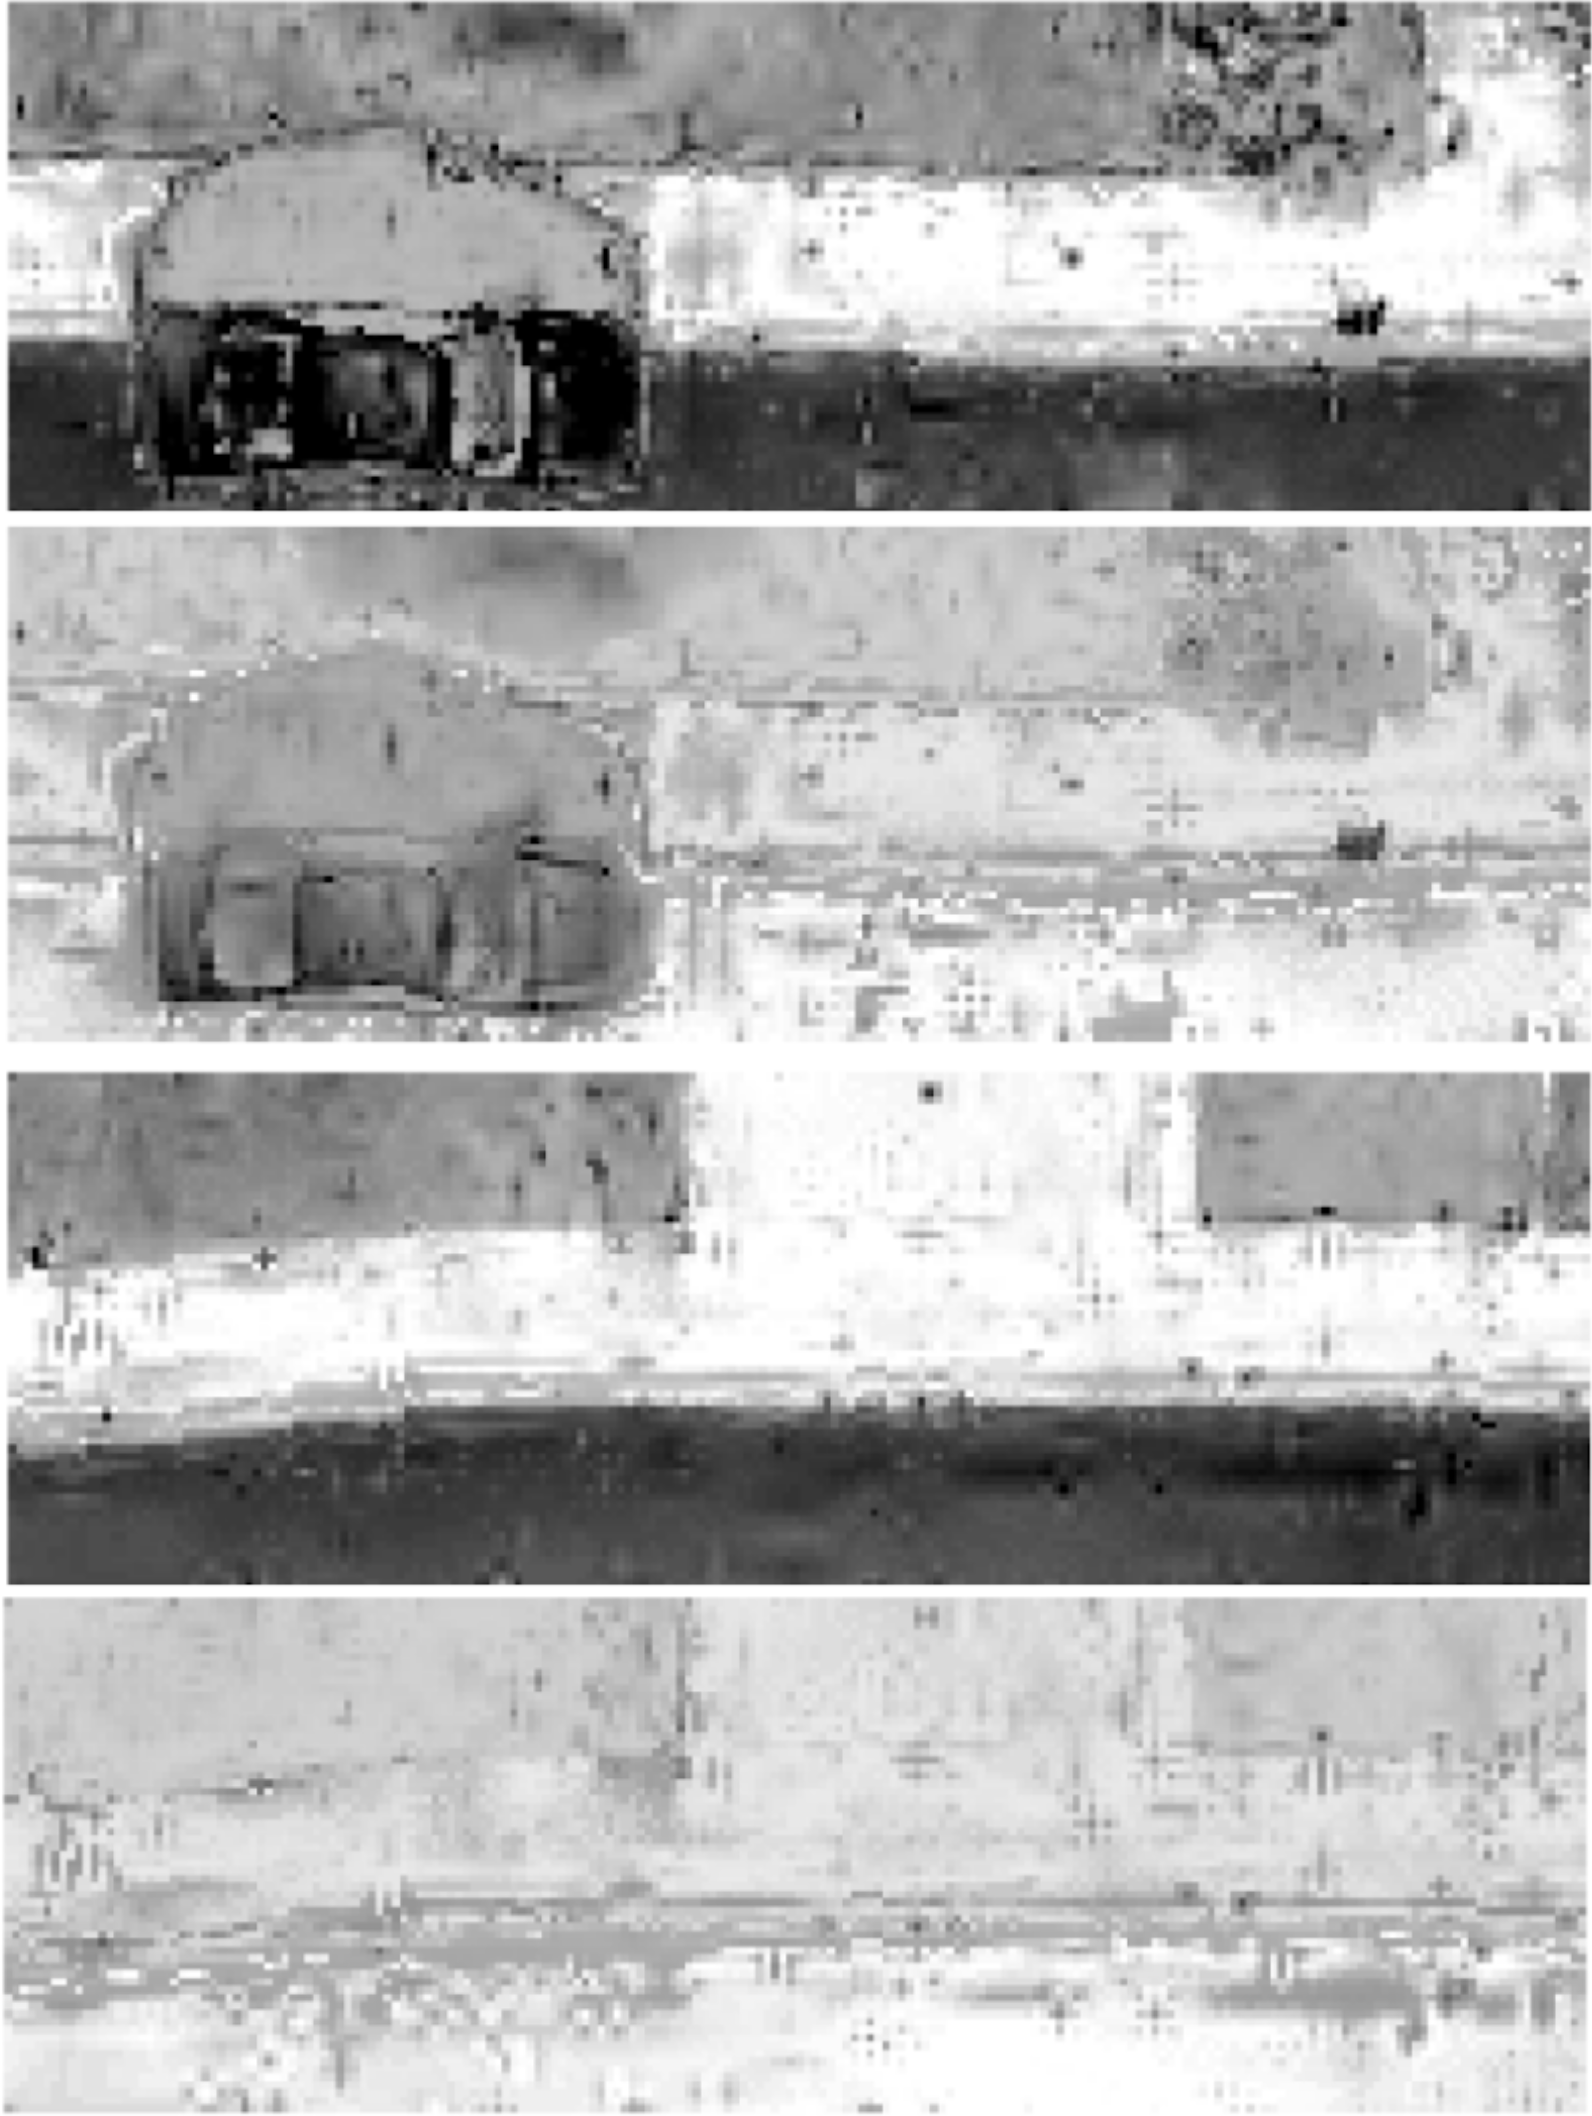
\includegraphics[width=0.8\textwidth]{Figures/GMM_needed.png}
    \caption[\ac{GMM} Result 1]{Example of GMMs on sample sidewalk. The first row and third row shows the foreground GMM for sample sidewalk, and the second row and fourth row shows the back-ground for simple sidewalk. We use grey-scale to show the changes of probabilities, where for foreground, white is more likely to be sidewalk, and black is not.}
    \label{fig:GMM_result}
\end{figure}


We aim to find a segmentation that combines \textit{shape} priors on the curvature and thickness of the ribbon-like features and also maximizes the likelihood of observing colors in the image. 
Let $\Lambda$ be a random variable for the event that a color $\lambda$ is observed in an image, and let $R$ indicate a random variable so that $R=1$ if a pixel is part of ribbon and $R=0$ if a pixel is not. A variety of approaches exist to learn the conditional probability $\Pr(\Lambda|R)$ of observing a color conditioned on whether a pixel within or outside of a ribbon \cite{hartigan1979algorithm, jordan1999introduction}. Many of these methods take as input a set of training examples in order to choose parameters for some model.  Our conjecture is that the initial estimate of our sidewalk's mid-line, while perhaps not perfect, is much more likely to cover pixels that are part of a sidewalk than the pixels at the edge of the ribbon image. 

We use this assumption to estimate the probability that a pixel is part of a ribbon conditioned on its color. Let $k_n$ be parameter that describes the radius around the medial curve that we will consider to be part of the ribbon with very high confidence. Let $k_f$ indicate a distance from the medial curve that we consider very unlikely to be part of the ribbon. Finally, let $k_W$ indicate maximum value of $t$ to consider when learning the distribution of colors in a ribbon image.  We model the distribution of colors within the sidewalk as a Gaussian Mixture Model of $k_g=4$ full-co-variance gaussian distribution and we model the distribution of colors outside of the ribbon as a mixture $2k_g$ Gaussian since we expect more variation and complexity in this zone. As shown in figure \ref{fig:GMM_result}, given an initial estimate for the set of colors inside or outside of the ribbon, we estimate the weights and co-variances of the Gaussians using the \ac{EM-GMM} \cite{sridharan2014gaussian} algorithm. 


\section{A Lattice Representation of the Problem} 
We represent the solution to this problem as graph where each node represents a point that may lie on the middle of a ribbon with a different width, and edges connect each node to a node that may have preceded it on a path. 

We will assume that widths may take on values from a set of predefined odd numbers (so that there is always a pixel in the center) 
Then the negative log-likelihood of for a particular pair of values $t_s$ and $r_s$ at a single row $(s)$ is 

\begin{align}
\rownll(s, t_s, r_s) &= -\log \Pr(r_s, t_s)  + \sum_{t} \pixelnll(s,t, t_s, r_s) \\
\pixelnll(s, t, t_s, r_s) &= 
\begin{cases}
 -\ln\Pr(\image(\x_{s,t})|\x_{s,t} \in R) &\text{if } t\in [t_s-r_s, t_s+r_s]\\
 -\ln\Pr(\image(\x_{s,t})|\x_{s,t}\not\in R) &\text{if } t\not\in[t_s-r_s, t_s+r_s]
\end{cases}
\end{align}

which combines the probabilities of seeing each color at offset $s$ in the ribbon image conditioned on whether the color is inside or outside of the ribbon. However, we assume ribbons are continuous with respect to the position of their mid-line and their thickness, likelihood of the most probable path up to offset $s$ is 

\begin{align}
\ribbonnll(s, t_s, r_s) &=  \begin{cases}
-\log \Pr(r_s, t_s) & \text{if } s = 0\\
   \begin{aligned}
   & \rownll(s, t_s, r_s) \\ 
   & + \displaystyle\max_{\delta_t,\delta_r} [p(\delta_t, \delta_r)+\ribbonnll(s-1, t_s+\delta_t, r_s+\delta_r)]
   \end{aligned} & \text{if } s > 0.\\
\end{cases}
\end{align}

The quantity $p(\delta_t, \delta_r)$ is a penalty for changing direction or thickness, and could be set to the negative log likelihood of observing a change $\delta_t$ in position and a change $\delta_r$ in thickness.  For discrete choices of $\delta_t$ and $\delta_r$ these costs can be represented by number in a matrix.

% \begin{algorithm}
% \caption{A Dynamic programming approach predict edges for ribbon-like feature}

% \begin{algorithmic}
% \State Initialize a matrix $A$ to same shape as ribbon image
% \For {each line of pixel $s$ in ribbon image}
%     \For{each possible pixel as $t_s$ in width of line}
%         \For{each pixel as $r_s$ in between $t_s$ and edge of line}
%             \State Store the returned probabilities from function D in $A[0, ts, rs]$
%             \If{not the first line pixel}
%                 \For {each $\delta_t and \delta_r \in \{-1, 0, 1\}$}
%                     \State Store max sum value from returned probability,
%                     \State $A[s-1, t_s+\delta_t, r_s+\delta_r]$ and penalty in $A[s, t_s, r_s]$
%                     \State Also store the value of $\delta_t$ and $\delta_r$
%                 \EndFor
%             \EndIf
%         \EndFor
%     \EndFor
% \EndFor


% \end{algorithmic}
% \end{algorithm}